\section{Results and Discussion}

To evaluate the effectiveness of our method on interactive face synthesis by sketching, we conducted extensive experiments with a wide range of handdrawn sketches and local editing. 
We develop an interactive interface for drawing sketches and displaying the generated photos in real time.


%In Sec.~\ref{sec:datasets}, we introduce how to produce our training and testing datasets(). 
%In Sec.~\ref{sec:augmentation}, we introduce the method of data augmentation aiming to alleviate the issue that the generated image has poor tolerance to the spatial position change of the input sketches. And we show the generation results of the model trained with augmented data. 
%In Sec.~\ref{sec:results}, we conduct comparative experiments on hand-drawn sketches between our methods and pix2pixHD baseline. We show that our method achieves a better fine-grained control on generated images.

%\paragraph{Datasets.}
\noindent
\textbf{Datasets.}
CelebA-HQ dataset contains 30k face images in resolution $1024\times1024$. All the face images are cropped and globally aligned according to face landmarks.
To produce paired training data of sketches and face images, we extracted 68 landmarks from each face image in the CelebA-HQ dataset, connect these landmark points in sequence, and draw lines in width of two pixels to synthesize contours as sketches.
%As the face photos in Celeba-HQ dataset are global aligned, so are the contours.
Those contours are more simple and clean than other types of synthetic sketches like edge maps~\cite{csagan} and mask edge maps~\cite{maskgan}. 
In our experiments, all the synthetic contour images and face images are resized into $512\times512$. 
After removing the photos for which landmark extraction fails, the training set contains 14,973 pairs of contour image and face photo, while the test set contains 4,992 pairs of contour and face photo. 

%\subsection{Data Augmentation}\label{sec:augmentation} 
The face photos of the CalebA-HQ dataset are precisely aligned based on facial landmarks. 
%Fig.~\ref{fig:average_face} shows an average face of all the synthesized contours. It shows that the facial features and facial contours of training data are basically in the same position, in other words, the training data is global aligned. 
This issue leads to degraded generalization ability of the model.
%
In order to imitate the human hand-drawn sketches, we apply random translation and rotation to the training contour images. 
Specifically, offsets randomly selected from $[-d,d]^2$ and angles randomly selected from $[-\theta,\theta]$ are applied to the training contours, where $d$ is the maximum offset and $\theta$ is the maximum angle.
We set $d=25$ and $\theta=7^\circ$ in our experiments. 
However, the training face photos are not translated or rotated because we expect the generated images to remain global aligned regardless of the spatial location of the input sketches.
Fig.~\ref{fig:data_augmentation} illustrates the comparative results between images generated before data augmentation and that after data augmentation. 
The quality of generated images after data augmentation is greatly improved compared when the input sketches deviate from the training examples spatially.

\begin{figure}[htb]
	\centering
	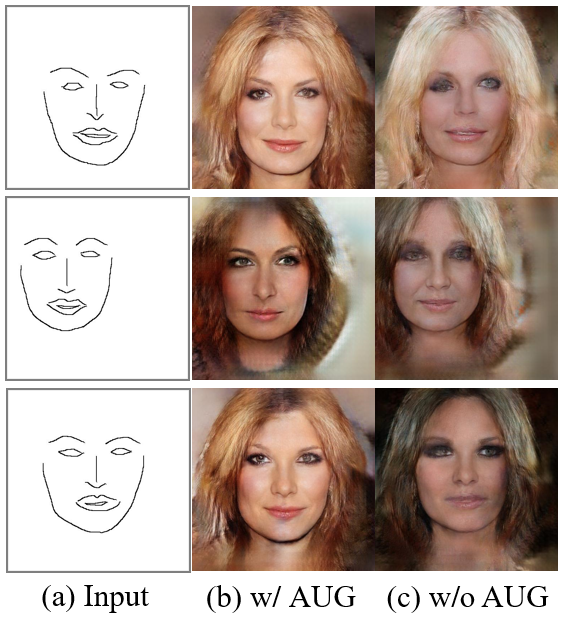
\includegraphics[width=0.35 \textwidth]{data_augmentation.png}
	\caption{Side-by-side comparison between images generated w/ and w/o data augmentation. }
	\label{fig:data_augmentation}
\end{figure}


\subsection{Qualitative Comparisons}\label{sec:results}
We conduct extensive experiments on different models with groups of elaborated hand-drawn sketches to verify the effect of instance normalization in generator on sketch-based face photo generation.


To explore how the amount of instance normalization layers in generator network affect the sketch-based face image generation quality, we train another model which takes the generator of pix2pixHD got rid of the first five instance normalization layers as its own generator. 
This model is refered to as $M_1$ for convenience.
We compare the face images generated by our model, $M_1$ and pix2pixHD. 
As you can see in Fig.~\ref{fig:ablation}, our model generates the most photorealistic images in contrast to the $M_1$ model which generates images lacking realism. 
It indicates that removing too many instance normalization layers in generator can weaken the model because training process is difficult to converge without normalization.
So it's reasonable for our model just to remove the first two instance normalization layers in generator. 
\begin{figure}[htb]
	\centering
	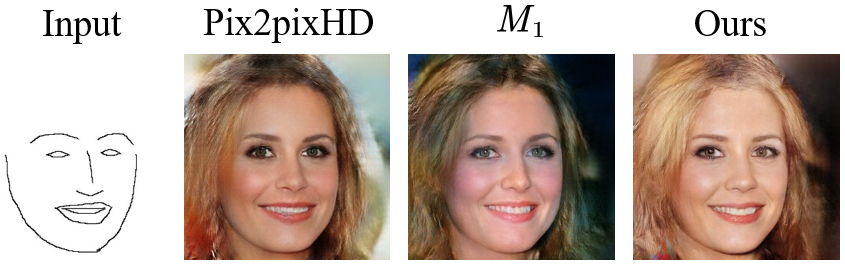
\includegraphics[width=\columnwidth ]{ablation.png}
	\caption{Comparison of results generated using different amount of instance normalization layers. }
	\label{fig:ablation}
\end{figure}  

Then we perform comparative experiments between our model and pix2pixHD baseline on hand-drawn sketches.
%Our model can preserve underlying information of input sketches so as to generate more plausible textures.
Results shown in Fig.~\ref{fig:compare_1} demonstrate that the baseline model frequently fails to synthesize realistic textures and many images generated by baseline model exhibit blurry artifacts.
We ascribe this issue to instance normalization that the generator creates blurry artifact to dominate the statistics to fool instance normalization layer. 
In contrast, the blurry artifacts alleviate obviously in our results when the first two instance normalization steps are removed from the generator.
Meanwhile, our results are more plausible with fine-grained textures due to our generator without the first two instance norm layers preserving more underlying information of input sketches.
\begin{figure}[htb]
	\centering
	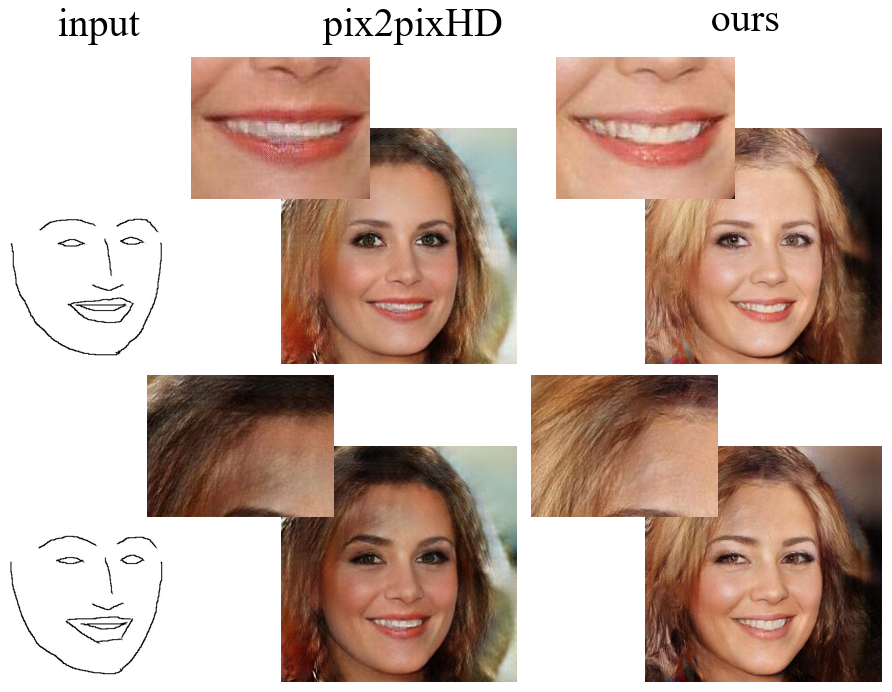
\includegraphics[width=0.45 \textwidth]{texture.png}
	\caption{Face images generated by our model and the baseline model with different mouth shape. The top row shows that the textures of teeth generated by pix2pixHD baseline are blurry, while our results have more realistic textures at the teeth area. The bottom row shows that some chaotic noises often emerge in the forehead area of the image generated by pix2pixHD baseline because the strokes of the mouth affect the other regions during feature embedding. In comparison, our model produces more globally realistic results.}
	\label{fig:compare_1}
\end{figure}

Our model can achieve fine-grained control on generated images. 
When we modify the strokes to represent different face attributes or change the overall face shapes in the input freehand sketches, the corresponding parts of images generated by our model change consistently while other areas remain unchanged. 
In comparison, using the baseline pix2pixHD model, modifying local strokes of sketches influences not only the content in corresponding areas but also the content in other areas in the generated images. 
Fig.~\ref{fig:compare_2} and Fig.~\ref{fig:compare_3}~ show several face images generated by our model and baseline model when changing lines of mouth and nose separately in sketches.
\begin{figure}[htb]
	\centering
	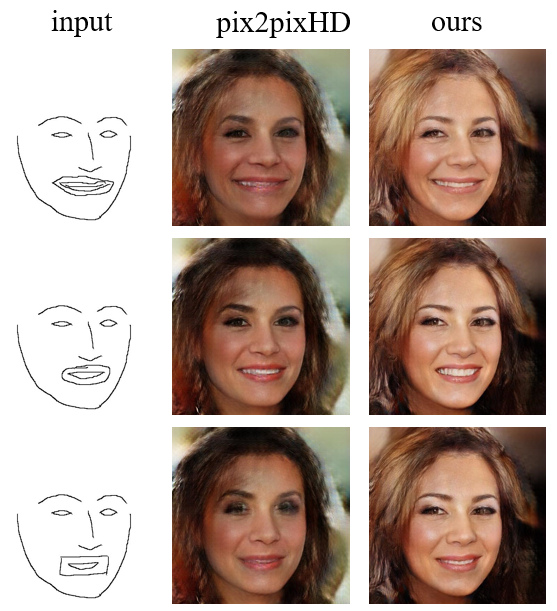
\includegraphics[width=0.4 \textwidth]{mouth_editing.png}
	\caption{Comparison between our model and baseline model tested with mouth-altered sketches. }
	\label{fig:compare_2}
\end{figure}
\begin{figure}[htb]
	\centering
	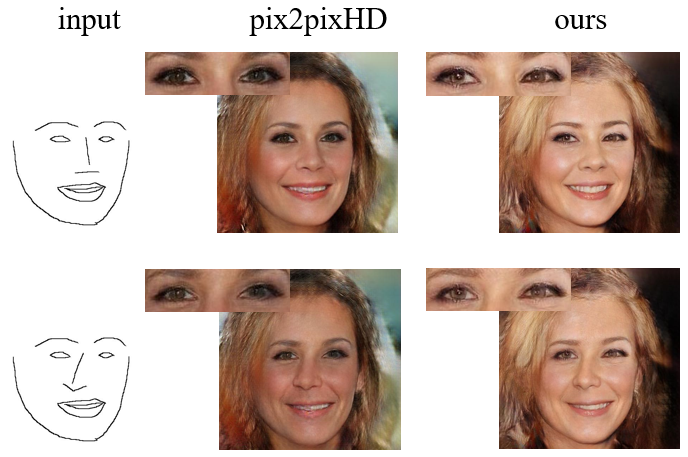
\includegraphics[width=0.45 \textwidth]{nose_editing.png}
	\caption{Comparison between our model and baseline model when the input sketches change locally at the nose shape.}
	\label{fig:compare_3}
\end{figure}
The results shown in first and second row of Fig.~\ref{fig:compare_2} demonstrate that the images generated by our model change obviously in mouth shape and preserve structure conformance with input sketches when modifying the lines of mouth in sketches. 
But the results generated by baseline model do not have an obvious change in mouth shape.
The results shown in Fig.~\ref{fig:compare_3} illustrate that the images generated by our model remain unchanged in other areas especially in eyes when altering the shapes of nose in sketches, but the images generated by baseline model change obviously in eyes direction. 
And as shown in the third row of Fig.~\ref{fig:compare_2}, the generation results of our model do not change except the mouth when modifying the mouth shape in sketches, while the generation quality of baseline model is degraded vastly especially in the eye area. 

\begin{table}[h]
	\centering	
	\caption{Results of user study.}
	\begin{tabular}{|c|c|c|}\hline
		& Baseline~\cite{pix2pixhd} & Ours \\\hline
		Preferance & $12.8\%$ & $\textbf{87.2\%}$\\\hline
	\end{tabular}
	\label{tab:user_study}
\end{table} 

Finally, user study is conducted to evaluate the perceptual generation quality of our model in comparison with baseline model. 
We organize 60 volunteers to join our experiment, each of them is tested with about 100 trials. The users are supposed to select images that are more realistic and match the input sketches better.  
The results reported in Table~\ref{tab:user_study} indicates that compared with baseline model, face images generated by our model are more plausible and controllable according to the test users. 

\section{Conclusion}
In this paper, we investigate the feature embedding in state-of-the-art image translation model on the sketch-based face image generation task.
We collect 11 groups of sketches with specific designs and utilize PCA to visually analyze the feature embedding for sketches.
The analysis indicates that the instance normalization tends to wash away the local shape information in the input sketches.
We improve the baseline image translation model by modifying the instance normalization layers in its generator.
The modified model effectively conveys fine-grained shape information through the image translation model and produces photorealistic face images that conforms with the input sketches on both local shape and global structure.
Extensive experiments demonstrate the effectiveness of our proposed method on the image quality and conformance with user intention in a sketch-based face image generation system.  